\documentclass[10pt]{article}
\usepackage[OE]{express}
\usepackage{float}
\usepackage{booktabs}
\providecommand{\e}[1]{\ensuremath{\times 10^{#1}}} 
\providecommand{\mb}[1]{\mathbf{#1}}
\providecommand{\mh}[1]{\mathbf{\hat{#1}}}
\providecommand{\bs}[1]{\boldsymbol{#1}} 
\providecommand{\intinf}{\int_{-\infty}^{\infty}}

\begin{document}
\title{Single-molecule orientation determination with multiview polarized
  illumination: modeling and microscope design}

\author{Talon Chandler,\authormark{1,*} Shalin Mehta,\authormark{2} Hari Shroff,\authormark{3,4} Rudolf Oldenbourg,\authormark{2, 5} and Patrick J. La Rivi\`ere\authormark{1, 4}}
\address{\authormark{1}University of Chicago, Department of Radiology, Chicago, Illinois 60637, USA\\
  \authormark{2}Marine Biological Laboratory, Bell Center for Regenerative Medicine, Woods Hole, Massachusetts, USA\\
  \authormark{3}Section on High Resolution Optical Imaging, National Institute
  of Biomedical Imaging and Bioengineering, National Institutes of Health,
  Bethesda, Maryland 20892, USA\\
  \authormark{4}Whitman Center, Marine Biological Laboratory, Woods Hole,
  Massachusetts 02543, USA\\
  \authormark{5}Brown University, Department of Physics, Providence, Rhode
  Island 02912, USA}
\email{*talonchandler@talonchandler.com} %% email address is required

%%%%%%%%%%%%%%%%%%% abstract and OCIS codes %%%%%%%%%%%%%%%%
\begin{abstract*}
  We investigate the use of polarized illumination in multiview microscopes for
  determining the orientation of single molecules. First, we relate the
  orientation of single molecules to measurable intensities in multiview
  microscopes and develop an information theoretic metric---the solid angle
  uncertainty---to compare the ability of multiview microscopes to estimate the
  orientation of single molecules. Next, we compare a broad class of microscopes
  using this metric---single- and dual-view microscopes with varying
  illumination polarization, illumination numerical aperture (NA), detection NA,
  obliquity, asymmetry, and exposure. We find that multiview microscopes are
  better at determining the orientation of single molecules than single-view
  microscopes. We also find that choosing a small illumination NA and a large
  detection NA are good design choices, that multiview widefield microscopes can
  benefit from oblique illumination and detection, and that asymmetric NA
  microscopes can benefit from exposure asymmetry.
\end{abstract*}

\ocis{(110.0110) Imaging systems; (180.2520) Fluorescence microscopy; (180.0180)
  Microscopy; (180.6900) Three-dimensional microscopy; (130.5440)
  Polarization-selective devices; (260.5430) Polarization.}

%%%%%%%%%%%%%%%%%%%%%%% References %%%%%%%%%%%%%%%%%%%%%%%%%
%% Comment before submission
\bibliography{paper}
\bibliographystyle{osajnl}

%% Copy .bbl and uncomment these before submission
% \begin{thebibliography}{99}
% \bibitem{gallo99} K. Gallo and G. Assanto, ``All-optical diode based on second-harmonic generation in an asymmetric waveguide,'' \josab {\bfseries 16}(2), 267--269 (1999).
% \end{thebibliography}

\section{Introduction}
The orientation of single molecules is a valuable reporter for biological
processes. By imaging biological samples with fluorescent probes that are fixed
to known structures, researchers have studied the dynamics of motor proteins
\cite{peterman2001, forkey2003}, DNA \cite{backer2016}, actin \cite{mehta2016},
septin \cite{demay2011, mcquilken2017}, and membranes \cite{anantharam2010}. The
number of techniques available to biologists for measuring the orientation of
single molecules in live cells is continually expanding. A recent review
\cite{backlund2014} identified three major categories of single molecule
orientation determination techniques:

\textbf{Spatial variation of emission} techniques image single molecules and use
the spatial distribution of intensity in the back focal plane \cite{lieb2004} or
in the image plane \cite{backer2014} to estimate their orientation. The best
techniques in this category use defocusing or phase masks in the back focal
plane to encode orientation and position information in the image
\cite{agrawal2012}. These techniques can estimate the orientation of
molecules in all orientations and only require a single frame, but they
require complex reconstruction algorithms, expensive high numerical aperture
(NA) optics, and sensitive detectors. 

\textbf{Spatial variation of illumination polarization} techniques vary the
polarization and intensity in the illumination path to excite molecules in
specific orientations in the focal volume \cite{debarre2004}. Although these
techniques can accurately estimate the orientation of molecules in all
orientations, they require scanning which makes these techniques too slow for
live cell imaging.

\textbf{Polarized illumination or detection} techniques exploit the anisotropic
absorption and emission pattern of single molecules to estimate their
orientation. By measuring the total intensity in the detector plane while
varying polarizer orientations on the illumination or detection path, the
orientation of the molecule can be estimated. These techniques are easy to
implement---changing the illumination or detection polarization is simple with a
polarization splitter \cite{mehta2016} or universal compensator
\cite{oldenbourg1995}---and the reconstruction methods are straightforward
\cite{fourkas2001, mehta2016, backer2016}. The main drawback is that these
techniques require several polarization frames to estimate the orientation of a
single molecule. Despite the requirement for multiple frames, polarized
illumination or detection methods are good choices for live cell imaging because
of their good combination of speed and ease of implementation.

The choice remains---is it best to put polarizers on the illumination path or
the detection path? Placing a polarizer in the illumination path lengthens
acquisition time because the polarizer needs to be changed for each polarization
frame, but polarized illumination provides the largest intensity differences
between molecules in different orientations. Placing polarizers in the detection
path doesn't slow down acquisition (multiple polarization frames can be
collected at once with a polarization splitter), but polarized detection
provides a smaller difference in intensity between molecules in different
orientations than polarized illumination. We are most interested in finding the
orientation of molecules with high precision, so polarized illumination is the
method we consider and extend in this paper.

All single molecule orientation determination methods suffer from some degree of
anisotropic orientation uncertainty, i.e., some molecular orientations cannot be
determined as precisely as others. In some cases the orientation cannot be
determined at all---the forward model can be degenerate for specific dipole
orientations \cite{fourkas2001, lu2008}. We feel that the importance of
isotropic orientation uncertainty has been underappreciated. To our knowledge,
the only authors who have considered anisotropic orientation uncertainty have
only analyzed a small set of molecular orientations instead of all orientations
\cite{agrawal2012}. Our view is that an ideal technique for determining the
orientation of single molecules can reconstruct the orientation with a small and
nearly uniform uncertainty for all molecule orientations.

Recently, there has been increasing interest in multiview microscopy techniques
for biological imaging \cite{wu2013, keller2015, wu2016, wu2017}. Multiview
microscopes offer two major advantages over single-view microscopes. First,
multiview microscopes can achieve nearly isotropic resolution compared to the
poor axial resolution of single-view microscopes. Second, multiview microscopes
can use light-sheet illumination to reduce phototoxicity without requiring
dedicated illumination optics. For example, if two orthogonal objectives are
focused on the same point, then both objectives can alternate roles as the
light-sheet illumination path and as the detection path. Light-sheet
illumination offers a major reduction of phototoxicity because a light sheet
only illuminates in focus regions while single-view microscopes illuminate out
of focus regions. Together, these advantages make multiview microscopes good
candidates for imaging live biological specimens for long periods.

In this work we explore the use of polarized illumination in multiview
microscopes for determining the orientation of single molecules. Existing
multiview microscopes can easily be outfitted with fast-switching polarizers
that do not degrade image quality, so polarized illumination is a natural way to
augment multiview microscopes for measuring the orientation of single
molecules. Furthermore, multiview microscopes can achieve nearly isotropic
resolution while delivering selective illumination. We hypothesize that
multiview microscopes will also provide a small and uniform orientation
uncertainty for single molecules in all orientations. In section \ref{methods}
we develop the required theory for polarized illumination microscopy and develop
information theoretic metrics to compare multiview microscopes. In section
\ref{results} we compare the results for a wide range of multiview microscope
designs. Finally, in section \ref{discussion} we discuss the results and their
impact on polarized multiview microscope design.

\section{Methods}\label{methods}
In this section we develop a method to compare multiview polarized illumination
microscopes for the task of reconstructing molecular orientations. In sections
\ref{excitation}--\ref{forward} we develop the forward model for single-frame
microscopes with a fixed illumination and detection configuration. In section
\ref{designs} we list a variety of ways that single-frame microscopes can be
combined to create experimentally realizable multi-frame microscopes. Finally,
in section \ref{metrics} we develop metrics that we will use to compare
multi-frame microscopes.

Note our distinction between a \emph{frame} and a \emph{view}. A frame refers to
a single intensity measurement with a fixed polarizer setting, illumination
path, and detection path. Acquiring additional frames entails varying the
polarizer setting, illumination path, or detection path. A view refers to a
detection path, and multiview microscopes use multiple detection paths.

We use roman type for scalars, e.g., $\phi$, $\theta$; bold lowercase type for
vectors, e.g., $\mb{r}, \bs{\mu}$; hats for unit vectors, e.g.,
$\mh{r}, \hat{\bs{\mu}}$; and bold capital type for matrices, e.g.,
$\mb{R}, \mb{F}$.

\subsection{Absorption Efficiency}\label{excitation}
In this section we will calculate the \emph{absorption efficiency} of a single
molecule---the fraction of the incident power that is absorbed by the
molecule. Our approach is inspired by Fourkas \cite{fourkas2001}, but here we
calculate the absorption efficiency instead of the detection efficiency.

\begin{figure}[H]
\centering\includegraphics[width=\textwidth]{frames}
\caption{Coordinate systems for a) the absorption dipole moment
  $\hat{\bs{\mu}}_{\text{abs}}$, b) the polarizer transmission axis
  $\hat{\mb{e}}_{\text{exc}}$, and c) the dummy integration vector
  $\hat{\mb{r}}$.}
\label{fig:coordinates}
\end{figure}

We consider a single molecule with an absorption dipole moment
$\hat{\bs{\mu}}_{\text{abs}}$ that we express in spherical coordinates $\Theta$
and $\Phi$ (see Figure \ref{fig:coordinates}a)) as
\begin{align}
  \hat{\bs{\mu}}_{\text{abs}}(\Theta, \Phi) = \sin\Theta\cos\Phi\hat{\mb{x}} + \sin\Theta\sin\Phi\hat{\mb{y}} + \cos\Theta\hat{\mb{z}} \label{eq:mu}.
\end{align}
We place the molecule at the focal point of an ideal, aplanatic,
polarization-preserving objective with the optical axis aligned with the
$\mh{z}$ axis. Finally, we place a polarizer behind the objective with a
variable transmission axis $\hat{\mb{e}}_{\text{exc}}$ that we express as
\begin{align}
 \hat{\mb{e}}_{\text{exc}}(\phi_{\text{exc}}) = \cos\phi_{\text{exc}}\hat{\mb{x}} +
\sin\phi_{\text{exc}}\hat{\mb{y}},\label{eq:excfield}
\end{align}
where $\phi_{\text{exc}}$ is the angle between the transmission axis of the
polarizer and the positive $\mh{x}$ axis (see Figure
\ref{fig:coordinates}b)). We illuminate the polarizer with a beam of collimated
light propagating along the optical axis, so the electric field incident on the
objective is parallel with the transmission axis of the polarizer.

We denote the illuminated region of the objective by $\Omega$. If we use
unit vectors $\hat{\mb{r}}$ expressed in spherical coordinates $\theta$ and
$\phi$ (see Figure \ref{fig:coordinates}c)) as
  \begin{align}
   \hat{\mb{r}}(\theta, \phi) = \sin\theta\cos\phi\hat{\mb{x}} + \sin\theta\sin\phi\hat{\mb{y}} + \cos\theta\hat{\mb{z}}, 
  \end{align}
  then the region $\Omega$ can be expressed as
  \begin{align}
  \Omega = \{\phi, \theta\ |\ 0 < \phi \leq 2\pi, 0 < \theta \leq \alpha\},
  \end{align}
  where $\alpha$ is the angle between the optical axis and the most oblique
  illuminating ray. Equivalently, $\alpha$ can be expressed in terms of NA using
  \begin{align}
    \text{NA} = n\sin\alpha, 
  \end{align}
  where $n$ is the index of refraction of the sample medium. Note that the NA of
  the objective is always greater than or equal to the illumination NA because
  we can under fill the back aperture of the objective.
  
  The objective focuses the collimated illumination by applying a position-dependent
  rotation to the electric field which we model by multiplying the incident electric
  field $\hat{\mb{e}}$ by a position-dependent rotation matrix
  \begin{align}
  \mb{R}(\mh{r}) &= \begin{bmatrix} \cos\theta\cos^2\phi + \sin^2\phi & (\cos\theta -1)\sin\phi\cos\phi & -\sin\theta\cos\phi\\ (\cos\theta - 1)\sin\phi\cos\phi & \cos\theta\sin^2\phi + \cos^2\phi & -\sin\theta\sin\phi \\ \sin\theta\cos\phi& \sin\theta\sin\phi & \cos\theta \end{bmatrix} \label{eq:rot_mat}.
  \end{align}

  To find the absorption efficiency $\eta_{\text{abs}}$ of a single molecule if
  it were illuminated by a single ray, we take the unit incident electric field
  $\hat{\mb{e}}$, take the dot product with the absorption dipole moment, then
  take the modulus squared
    \begin{align}
      \eta_{\text{abs}} &= |\hat{\bs{\mu}}_{\text{abs}}\cdot\mh{e}_{\text{exc}}|^2. \label{eq:singleray}
    \end{align}

    To find the absorption efficiency of a single molecule under incoherent
    focused light, we integrate over all rays and divide by the total incident
    power which gives the vector expression
\begin{align}
  \eta_{\text{abs}} = \frac{\int_{\Omega}d\mh{r}|\hat{\bs{\mu}}_{\text{abs}}\cdot\mb{R}(\mh{r})\mh{e}_{\text{exc}}|^2}{\int_{\Omega}d\mh{r}}\label{eq:abs}. 
\end{align}

We substitute equations \ref{eq:mu}--\ref{eq:rot_mat} into equation
\ref{eq:abs}, evaluate the integrals, and simplify to express the absorption
efficiency in scalar notation as
\begin{align}
  \eta_{\text{abs}} &= D\{A + B\sin^{2}{\Theta} + C\sin^{2}{\Theta} \cos{[2 (\Phi - \phi_{\text{exc}}})]\}\label{eq:scalarabs}
\end{align}
where
\begin{subequations}
\begin{align}
  A &= \frac{1}{4} - \frac{3}{8} \cos{\alpha } + \frac{1}{8} \cos^{3}{\alpha }\\
  B &= \frac{3}{16} \cos{\alpha } - \frac{3}{16} \cos^{3}{\alpha }\\
  C &= \frac{7}{32} - \frac{3}{32} \cos{\alpha } - \frac{3}{32} \cos^{2}{\alpha } - \frac{1}{32} \cos^{3}{\alpha}\\
  D &= \frac{4}{3(1 - \cos\alpha)}.
\end{align}\label{eq:coefficients}%
\end{subequations}

At the beginning of this section we assumed that the molecule was located at the
focal point of the condenser. If the illumination objective is aplanatic and we
use K\"ohler illumination, then we can relax this assumption and the above
expressions are valid for molecules anywhere in the focal plane.

We also assumed that we used incoherent illumination, but we can extend these
results to light-sheet illumination that uses a scanned coherent laser. If we
illuminate the back aperture with a weakly focused laser beam and scan the laser
beam slowly---if the scan velocity is much less than the beam waist radius
divided by the coherence time---we can ignore longitudinal excitation and the
molecule will be excited as if a single plane wave was incident. Therefore, we
can find the absorption efficiency of a molecule under weakly focused scanned
laser illumination by taking the limit of equation \ref{eq:scalarabs} as
$\alpha \rightarrow 0$ (or by plugging equation \ref{eq:mu} and
\ref{eq:excfield} into equation \ref{eq:singleray}) giving
\begin{align}
  \eta_{\text{abs}} &= \sin^2\Theta\cos^2(\Phi - \phi_{\text{exc}}),
\end{align}
which is recognizable as Malus' law generalized to three dimensions. This means
that light-sheet illumination is approximately equivalent to widefield
illumination with a low NA. Notice that the absorption efficiency can take its
maximum range of values ($\eta_{\text{abs}} \in [0, 1]$) when $\alpha=0$.

\subsection{Detection Efficiency}\label{detection}
Fourkas calculated the detection efficiency of a single molecule when an
objective with a polarizer is aligned along the $\mh{z}$ axis
\cite{fourkas2001}. We use his expressions to calculate the detection efficiency
without a polarizer as
\begin{align}
  \eta_{\text{det}} = 2(A + B\sin^2\Theta). \label{eq:scalardet}
\end{align}
The detection efficiency only depends on $\Theta$, not $\Phi$, because there is
no detection polarizer. We have assumed that the absorption dipole moment is
equal to the emission dipole moment.

Note that $A$ and $B$ in equation \ref{eq:coefficients} are a factor of
$\frac{3}{2}$ larger than the expressions given by Fourkas. We found that
Fourkas' expressions were incorrectly normalized (the limit of
$\eta_{\text{det}}$ as $\alpha\rightarrow \pi/2$ should be 1), and the extra
factor of $\frac{3}{2}$ corrects the error. This correction does not affect
Fourkas' orientation reconstruction but it does mean that Fourkas' algorithm
under predicts the total emitted intensity by a factor of $\frac{3}{2}$.

Also note that the detection efficiency can take its maximum range of values
when $B$ takes its maximum value, i.e. when
$\alpha=\arccos\left(\frac{1}{\sqrt{3}}\right) \approx 54.7^{\circ}$. 

\subsection{Oblique Illumination and Detection}\label{oblique}
In sections \ref{excitation} and \ref{detection} we assumed that both the
illumination and detection objectives had $\mh{z}$ aligned optical axes, i.e.,
the same objective was used for illumination and detection. To extend the
forward model to oblique optical axes which allows for non-coincident
illumination and detection objectives, we express the dipole orientation in
rotated coordinates using the following expressions
\begin{align}
    \Theta' &= \arccos\left(\sin\psi\cos\Phi\sin\Theta + \cos\psi\cos\Theta\right)\label{eq:thetap}\\
  \Phi' &=
          \begin{cases}
            \arccos\left(\dfrac{\cos\psi\cos\Phi\sin\Theta - \sin\psi\cos\Theta}{\sqrt{1 - (\sin\psi\cos\Phi\sin\Theta + \cos\psi\cos\Theta)^2}}\right) \ \ \ &0 \leq \Phi < \pi  \\
            -\arccos\left(\dfrac{\cos\psi\cos\Phi\sin\Theta - \sin\psi\cos\Theta}{\sqrt{1 - (\sin\psi\cos\Phi\sin\Theta + \cos\psi\cos\Theta)^2}}\right) \ \ \ &-\pi \leq \Phi < 0\\
          \end{cases}
\end{align}
where $\psi$ is the angle of a right handed rotation about the $\mh{y}$ axis
that maps the $\mh{z}$ axis onto the new optical axis.

\subsection{Single-Frame Microscopes}\label{forward}
The detected intensity is the product of the the sample exposure
$I_{\text{tot}}$, the absorption efficiency, and the detection efficiency
\begin{align}
  I = I_{\text{tot}}\eta_{\text{abs}}\eta_{\text{det}}\label{eq:forward_frame}.
\end{align}
Equation \ref{eq:forward_frame} is the forward model for a \emph{single-frame
  microscope}. Figure \ref{fig:single-frame} shows the efficiencies from three
representative examples of single-frame microscopes.

The intensity measured by a single-frame microscope does not give us enough
information to reconstruct the orientation of a single molecule. Next, we
will consider combining several single-frame microscopes to create
\emph{multi-frame microscopes.}

\begin{figure}[H]
\centering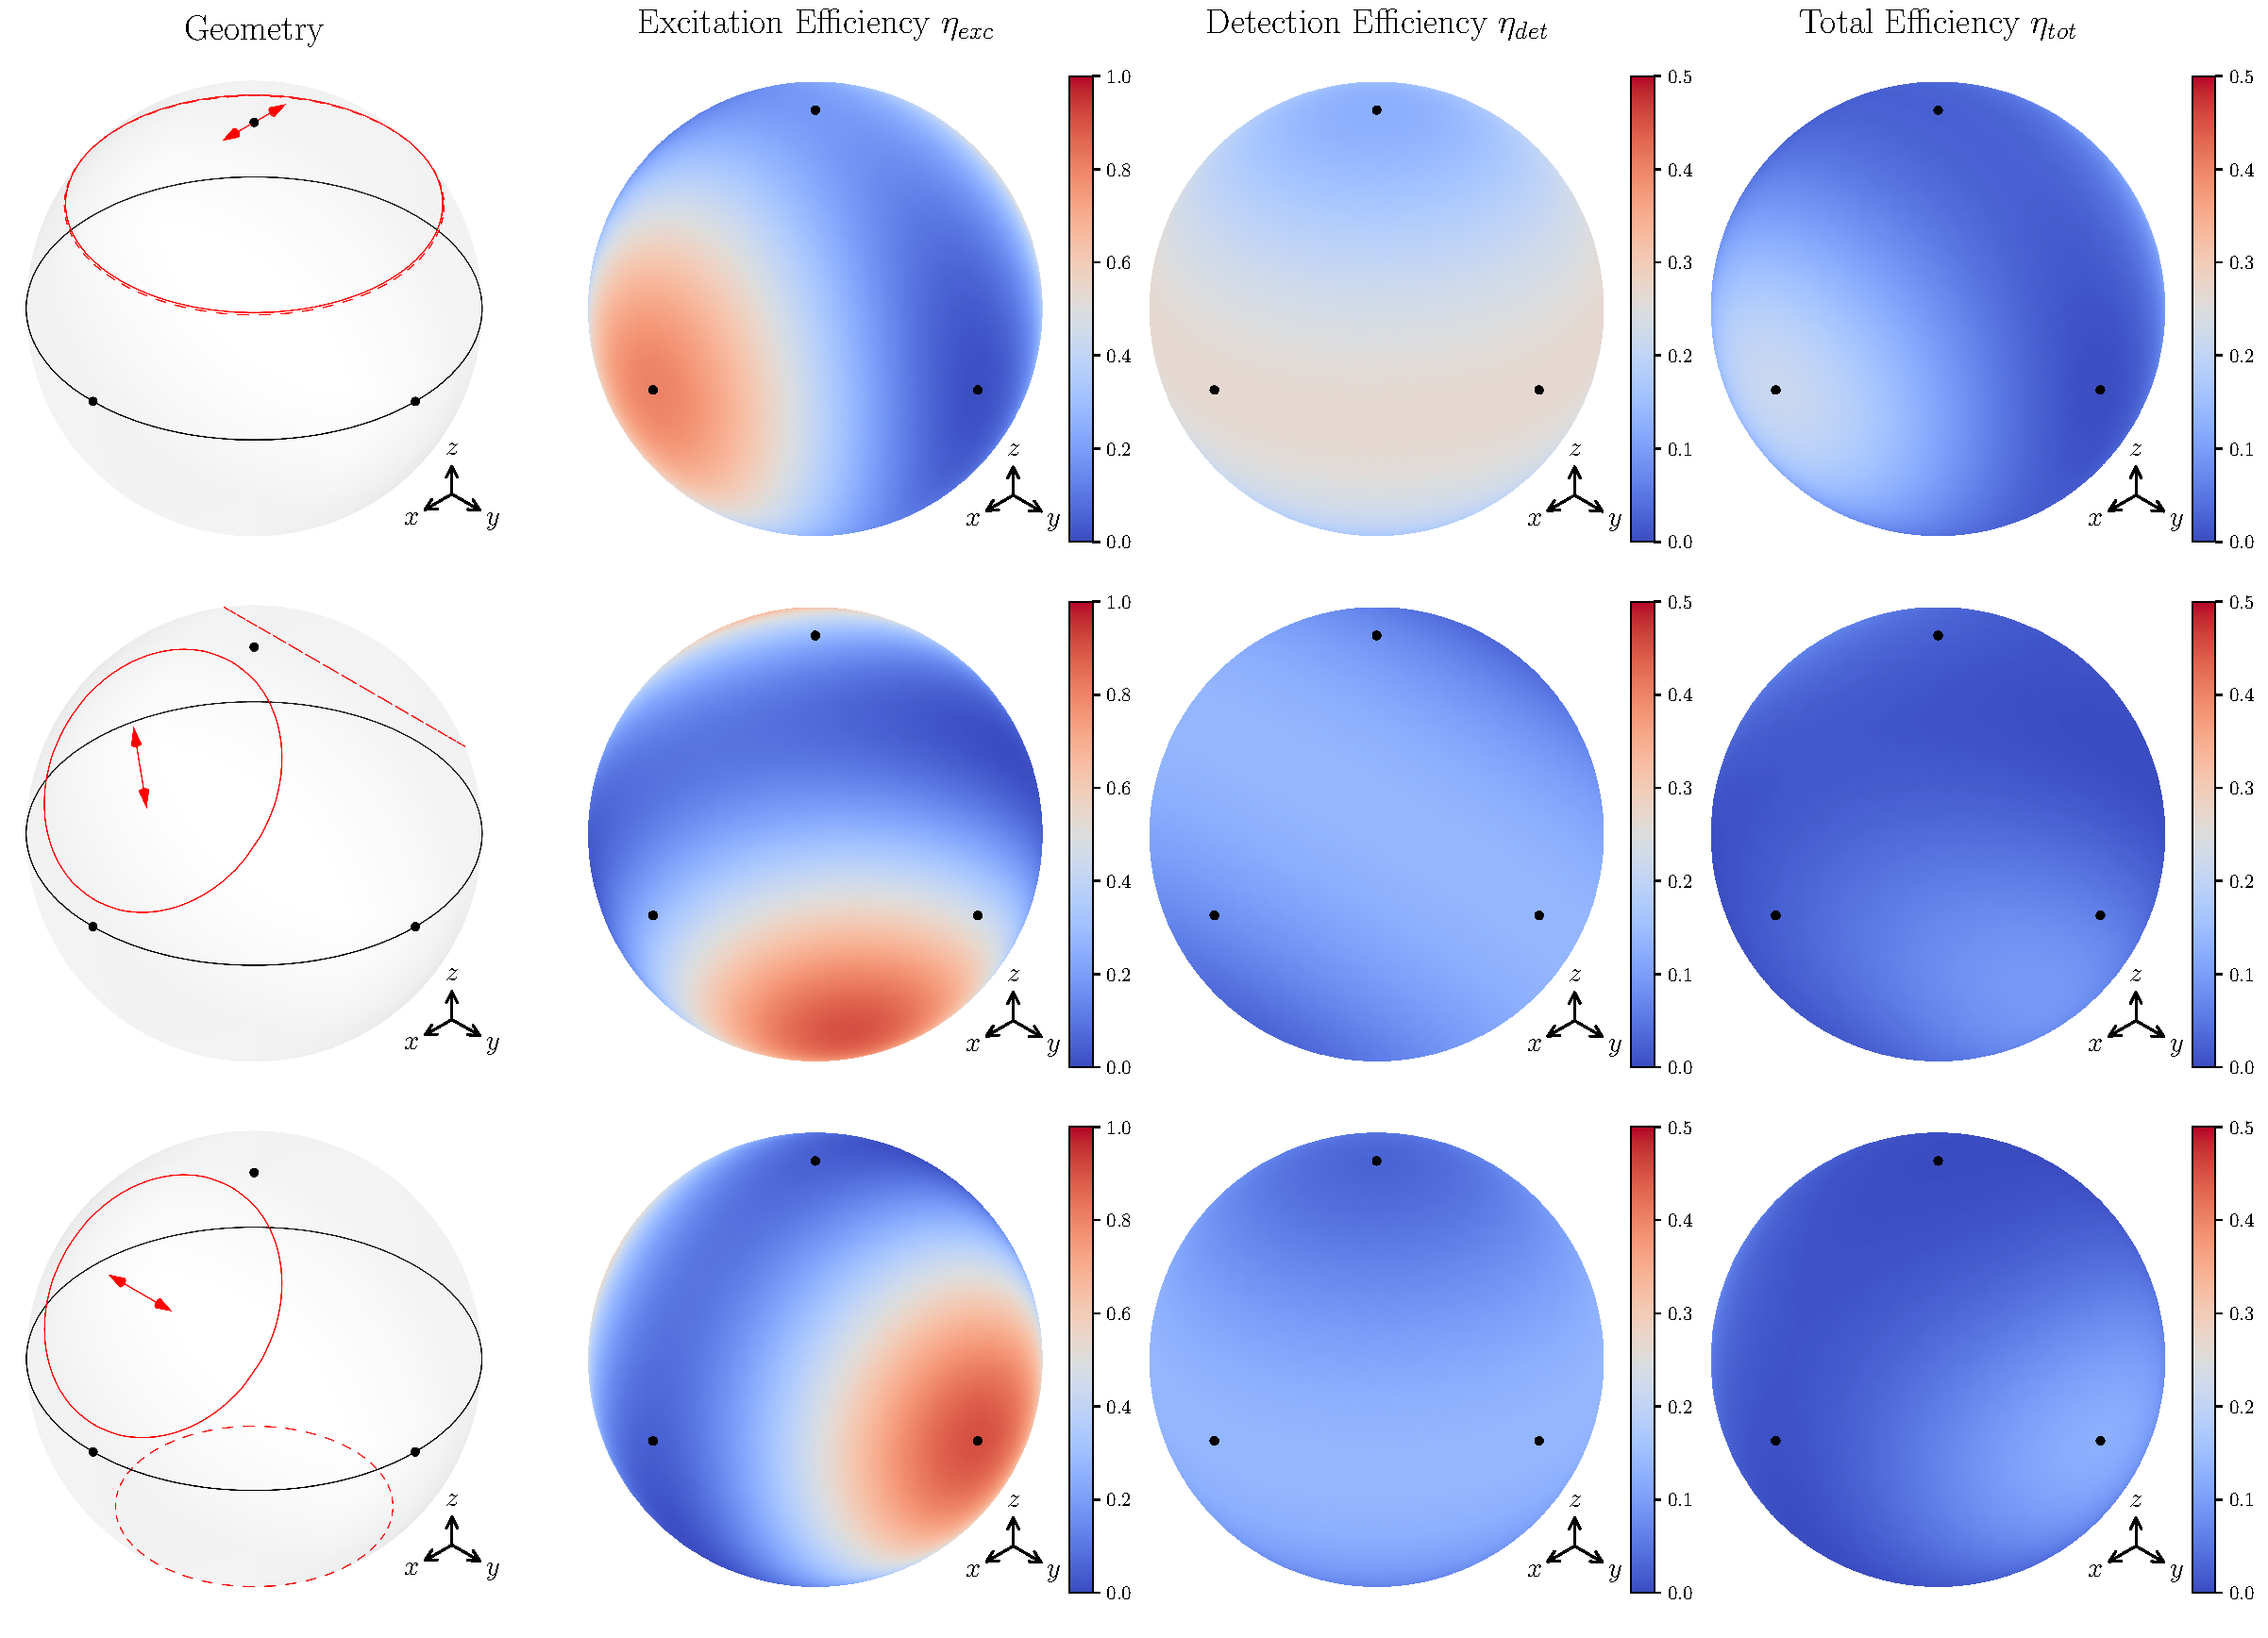
\includegraphics[width=\textwidth]{single-frame}
\caption{Representative examples of single-frame microscopes.\newline \newline
  \textbf{Columns left to right:} 1) schematics of single-frame microscopes
  where the solid line encloses the illumination solid angle, the dashed line
  encloses the detection solid angle, and the arrow indicates the transmission
  axis of the illumination polarizer; 2) the absorption efficiency, see equation
  \ref{eq:scalarabs}; 3) the detection efficiency, see equation
  \ref{eq:scalardet}; (4) the total efficiency, the product of the absorption
  and detection efficiencies.\newline \newline \textbf{Rows top to bottom:} 1)
  coincident illumination ($\text{NA} = 1.1$ with $x$-polarized light) and
  detection (NA = 1.1); 2) non-coincident orthogonal illumination
  ($\text{NA} = 0.8$) and detection ($\text{NA} = 0.8$); 3) non-coincident
  135${}^{\circ}$-separated illumination ($\text{NA} = 0.8$) and detection
  ($\text{NA} = 0.8$). All simulations use $n=1.33$.}
  \label{fig:single-frame}
\end{figure}


\subsection{Multi-Frame Microscopes}\label{designs}
One way to collect multiple frames is to add a universal compensator to the
illumination arm and rapidly select the incident polarization by changing
$\phi_{\text{exc}}$ \cite{oldenbourg1995}. All of the multi-frame microscopes we
will consider in this paper use four frames per view with the illumination
polarization separated by 45${}^{\circ}$.

We also consider several dual-view designs. We evaluate two-view designs that
allow for illumination and detection from both objectives (see \cite{wu2013} for
a dual-view design). In all cases we consider the effect of varying the
illumination and detection numerical aperture. We also consider asymmetric NA
designs (see \cite{wu2017} for an asymmetric NA design) and the effect of
asymmetric sample exposures. Note that we use the word \emph{symmetry} to refer
to dual-view designs with objectives that are identical and the word
\emph{asymmetry} to refer to dual-view designs with objectives that have a
different NA or sample exposure.

All multiview microscopes are subject to steric constraints---the objectives
must not collide with the cover slip or each other. We only consider microscope
designs that meet these criteria.

\subsection{Evaluation Metrics}\label{metrics}
Our goal is to evaluate the ability of a microscope design to estimate the
orientation of a single molecule (via parameters $\Theta$ and $\Phi$) from
intensity data.

A common way to evaluate the ability to estimate the parameters $\Theta$ and
$\Phi$ from the data is to calculate the Cramer-Rao lower bound (CRLB) for each
parameter \cite{kay1993}. The CRLBs are given by the diagonal elements of the
inverse of the Fisher information matrix, and they give the minimum variance of
an unbiased estimator for each parameter. For each microscope design and
molecule orientation we calculate the Fisher information matrix. If the
intensity is Poisson distributed the Fisher information matrix is given by
\begin{align}
  \mb{F} &= \sum_{k=1}^N \frac{1}{I_k}
  \begin{bmatrix}
    \dfrac{\partial I_k}{\partial \Theta}\dfrac{\partial I_k}{\partial \Theta}&\dfrac{\partial I_k}{\partial \Theta}\dfrac{\partial I_k}{\partial \Phi}\\\\
    \dfrac{\partial I_k}{\partial \Theta}\dfrac{\partial I_k}{\partial \Phi}&\dfrac{\partial I_k}{\partial \Phi}\dfrac{\partial I_k}{\partial \Phi}\\    
  \end{bmatrix}
\end{align}
where $I_k$ is the intensity measured in the $k$th frame of an $N$-frame
microscope. Agrawal et. al. used the square root of the product of the CRLBs
multiplied by the Jacobian determinant,
$\sin\Theta\sqrt{\mb{F}^{-1}_{0,0}\mb{F}^{-1}_{1,1}}$, to find the area of
uncertainty in parameter space \cite{agrawal2012}.

CRLBs and the associated area of uncertainty are parametrization dependent,
i.e., if we choose a different coordinate system these metrics will change. We
would like to compare microscope designs without choosing a parametrization, so
instead we use
\begin{align}
  \sigma_{\Omega} &\equiv \sin\Theta\sqrt{\text{det}\{\mb{F}^{-1}\}}
\end{align}
as our evaluation metric. We calculate the determinant of the inverse Fisher
information matrix---a parametrization-independent value called the
\emph{generalized variance} \cite{anderson1958}---take the square root, then
multiply by the Jacobian determinant, $\sin\Theta$. We call $\sigma_{\Omega}$
the \emph{solid-angle uncertainty} because it has units of steradians and is a
parametrization independent measure of the orientation uncertainty.

For each multi-frame microscope we calculate $\sigma_{\Omega}$ at 10,000
approximately equally spaced points on the unit sphere. A desirable microscope
design will have a small solid-angle uncertainty that is uniform for all
molecule orientations. The most straightforward way to find the location and
scale of the solid-angle uncertainty is to use the mean and variance,
respectively. However, because the solid-angle uncertainty admits extremely
large values that can change the mean and variance dramatically depending on the
sample points, we use the median and median absolute deviation (MAD)---the
median of the data's absolute difference from the median---as robust
alternatives to the mean and variance.

To compare multi-frame microscopes with different numbers of frames fairly, we
kept the total exposure to the sample constant by choosing
$I_{\text{tot}} = \frac{4000}{N}$. Note that $I_{\text{tot}}$ is a measure of
exposure to the sample, not the detected intensity or the total intensity
emitted by the molecule.

\section{Results}\label{results}
Figure \ref{fig:single-arm} shows our results for single-view designs where a
single objective is used for illumination and detection. We swept through the
illumination and detection NA while keeping the sample exposure constant, and we
found that the lowest median and MAD of the solid-angle uncertainty occurs with
a small illumination NA and a large detection NA where
$\alpha \approx 57.4^{\circ}$. A small illumination NA maximizes the range of
absorption efficiencies, while a large detection NA maximizes the number of
detected photons and the range of the detection efficiencies. Note the relative
importance of illumination and detection NAs---reducing the illumination NA (an
inexpensive modification requiring under filling the back aperture) improves the
solid angle uncertainty much less than increasing the detection NA (an expensive
modification requiring a higher NA objective). Also note in Figure
\ref{fig:single-arm}b) that single-view designs suffer from high orientation
uncertainty when the molecules are oriented along the optical axis (the
molecules are not efficiently excited), near the transverse plane (it is
ambiguous whether the molecule is oriented above or below the transverse plane),
and near the polarizer orientations (it is ambiguous whether the molecule is on
either side of the polarizer orientation).

\begin{figure}[htbp]
\centering\includegraphics[width=\textwidth]{single-arm}
\caption{Single-view microscope with varying illumination and detection
  NA. a) Schematic of a single-arm four-frame epi-illumination microscope. The
  red arrows indicate the four illumination polarization orientations---one for
  each frame. b) Solid angle uncertainty for the microscope in a). c) Median of
  the solid-angle uncertainty as a function of illumination and detection NA. d)
  MAD of the solid-angle uncertainty as a function of illumination and detection
  NA. The microscope in a) and b) is indicated by a cross in c) and d).}
\label{fig:single-arm}
\end{figure}

Figures \ref{fig:symmetric-widefield} and \ref{fig:double-arm} show our results
for dual-view symmetric widefield designs. We illuminate from one objective and
detect from the other for four polarization frames, then we repeat the
polarization frames with the same objectives in reversed roles. In Figure
\ref{fig:symmetric-widefield} we sweep through the NA of both objectives and the
angle between the objectives while considering steric constraints. Note how
adding a second view removes the high uncertainty region in the transverse
plane. The dual-view microscope still has high uncertainty regions near the
optical axes, but the uncertainty is reduced by almost two orders of magnitude
compared to the single-view microscope. We find that the lowest median of the
solid-angle uncertainty occurs with the largest possible NA objectives. We also
find that increasing NA always lowers the MAD, but orthogonal arms are not
always best. At large NA, it is advantageous to move the objectives together or
against the cover slip. Given the high uncertainty in the transverse plane for a
single-view shown in Figure \ref{fig:single-arm}b), we can see why oblique views
perform better than orthogonal views---oblique views are complementary because
the regions of high orientation uncertainty from each view do not overlap.

\begin{figure}[htbp]
\centering\includegraphics[width=\textwidth]{symmetric-widefield}
\caption{Dual-view symmetric widefield designs with varying NA and angle between
  objectives. a) Schematic of the microscope. We illuminate with the first objective
  (red solid) and detect from the second objective (red dashed). Then we
  illuminate from the second objective (blue solid) and detect from the first
  objective (blue dashed). b) Solid angle uncertainty for the microscope in
  a). c) Median of the solid-angle uncertainty as a function of NA and the angle
  between the objectives. d) MAD of the solid-angle uncertainty as a function of NA
  and the angle between the objectives. The microscope in a) and b) is indicated
  by a cross in c) and d). e) Median of the solid-angle uncertainty as a
  function of the angle between the objectives when NA=0.6. f) MAD of the
  solid-angle uncertainty as a function of the angle between the objectives when
  NA=0.6. The profile in e) and f) is taken along the green line in c) and d).}
\label{fig:symmetric-widefield}
\end{figure}

Figure \ref{fig:double-arm} shows our results when we used a dual-view symmetric
orthogonal widefield design and varied the illumination and detection NA. Our
results are similar to the single-view case in Figure \ref{fig:single-arm}. We
find that the best designs use a small illumination NA (like light-sheet
illumination) and a large detection NA where $\alpha \approx 57.4^{\circ}$. This
means that dual-view light-sheet illumination geometries are an excellent choice
for uniformly reconstructing the orientation of single molecules.

\begin{figure}[htbp]
\centering\includegraphics[width=\textwidth]{double-arm}
\caption{Dual-view symmetric orthogonal widefield designs with varying
  illumination and detection NA. a) Schematic of the microscope. b) Solid angle
  uncertainty for the microscope in a). c) Median of the solid-angle uncertainty
  as a function of illumination and detection NA. d) MAD of the solid-angle
  uncertainty as a function of illumination and detection NA. The microscope in
  a) and b) is indicated by a cross in c) and d).}
\label{fig:double-arm}
\end{figure}

Figure \ref{fig:asymmetric-double} shows our results for dual-view asymmetric
light-sheet illumination designs. We used light-sheet illumination on both sides
and kept the objectives orthogonal so that the light sheet from one objective
illuminates the focal plane of the other objective. We made the objectives
as large as possible so that both objectives would touch the cover slip and each
other ($\alpha_1 + \alpha_2 = 90$ in Figure \ref{fig:asymmetric-double}a)). We
swept through the NA asymmetry and the sample exposure asymmetry while keeping
the total sample exposure constant, and found that symmetric designs are at a
local minimum of the median and MAD of the solid-angle uncertainty. We also
found that at extreme asymmetries where the exposure from the low NA arm is much
larger than the exposure from the high NA arm (top-left and bottom-right corners
of Figures \ref{fig:asymmetric-double}c) and d)) the median and MAD are
comparable to the symmetric light-sheet microscope. This means that if a very
high NA objective is available and a low NA objective can provide light sheet
illumination, this microscope will perform comparably with a dual-view
microscope with two objectives of medium NA. Figure \ref{fig:asymmetric-double}
also shows that designs with slightly asymmetric NA can trade off a low
solid-angle uncertainty median for a low solid-angle uncertainty MAD by changing
the sample exposure ratio.

\begin{figure}[htbp]
  \centering\includegraphics[width=\textwidth]{asymmetric-double}
  \caption{Dual-view asymmetric light-sheet illumination designs with varying NA and
    sample exposure asymmetry. a) Schematic of the microscope. b) Solid angle
    uncertainty for the microscope in a). c) Median of the solid-angle
    uncertainty as a function of NA and sample exposure asymmetry. d) MAD of the
    solid-angle uncertainty as a function of NA and sample exposure
    asymmetry. The microscope in a) and b) is indicated by a cross in c) and
    d).}
\label{fig:asymmetric-double}
\end{figure}

Table 1 shows a summary of our evaluation metrics for the best microscopes in
each class. The single-view widefield microscope with a large illumination NA
and high detection NA has the lowest solid-angle uncertainty median but the
largest max. The dual-view oblique symmetric widefield with an intermediate NA
performs reasonably well on all three metrics, while the dual-view orthogonal
symmetric light sheet with the largest possible detection NA performs very well
on all three metrics.

\begin{table}[ht!]
\centering
\caption{Comparison of the best designs in each class of microscope. All values
  are in steradians.}
\begin{tabular}{llll}
  \toprule
Microscope Type&Max\{$\sigma_{\Omega}$\}&Median\{$\sigma_{\Omega}$\}&MAD\{$\sigma_{\Omega}$\}\\ \midrule
Single-view widefield (NA${}_\textrm{ill}$=0, NA${}_\textrm{det}$=1.1)&3.04$\times 10^{0}$&8.20$\times 10^{-4}$&1.40$\times 10^{-4}$ \\ 
Dual-view oblique symmetric widefield (NA=0.6, $\beta$=53${}^{\circ}$)&1.35$\times 10^{-1}$&4.49$\times 10^{-3}$&9.17$\times 10^{-4}$\\
Dual-view orthogonal symmetric light-sheet (NA=0.94)&3.13$\times 10^{-3}$&1.28$\times 10^{-3}$&1.14$\times 10^{-4}$\\
\bottomrule
\end{tabular}
\end{table}

\section{Discussion and Conclusions}\label{discussion}
In this work we have developed a model to predict the intensities measured by
polarized illumination microscopes in a wide range of geometries, developed
metrics to measure the ability of a microscope design to estimate the
orientation of single molecules, and used these metrics to compare a wide
range of microscope designs. Our main result is a short list of design
heuristics that can be used to design polarized-illumination single-molecule
orientation microscopes:
\begin{itemize}
\item All microscopes benefit from a small illumination NA and a large detection
  NA with $\alpha \approx 57.4^{\circ}$.
\item Dual-view microscopes outperform single-view microscopes, and dual-view
  microscopes remove the high uncertainty region in the transverse plane of
  single-view microscopes.
\item High NA dual-view widefield microscopes are best when the two views are
  oblique. Oblique views are complementary because their high uncertainty
  transverse planes do not overlap.
\item Symmetric NA dual-view orthogonal light-sheet microscopes provide a good
  compromise between cost, solid-angle uncertainty median, and solid-angle
  uncertainty MAD. Asymmetric NA dual-view orthogonal light-sheet microscopes
  can improve the solid-angle uncertainty median or MAD by changing the sample
  exposure ratio between the two views.
\end{itemize}

Our results are limited in several ways. First, we only consider single
molecules in homogeneous environments. We ignore light reflected from the cover
slip and any other inhomogeneities in the sample. If we considered light
reflected from the cover slip we expect that the results would put a lower
weighting on large detection NAs because we would collect more light. Second, we
only considered ideal, polarization preserving, aplanatic objectives. In
practice, these conditions are not always satisfied and the power from high NA
rays is apodized by a factor of $\frac{n}{\cos\Theta}$
\cite{nov2006}. Therefore, our results are most accurate for low NA rays and get
progressively worse for high NA rays, although our major conclusions would not
change if we included this apodization factor. The main advantage of ignoring
apodization is the tractability of the problem---we have provided approximate
closed-form solutions for the illumination and detection efficiencies that have
allowed us to draw useful design conclusions.

To compare the microscopes in this paper we used a fixed sample exposure. We
think that this is the fairest way to compare microscopes with different numbers
of frames. However, in cases where sample exposure and time are not an issue it
may be more useful to compare microscopes with the same detection exposure per
frame. This comparison would favor multiple frame microscopes even more that the
results in this paper, because equal detection exposure per frame would improve
photon counting statistics.

We have considered single- and dual-view microscopes in a variety of cases, but
more multiview microscopes can be analyzed with the framework we have
developed. Wu et. al. have developed a three-view design with a third objective
below the cover slip\cite{wu2016}. Light-field detection schemes are also a type
of multiview microscope\cite{levoy2006}, and we plan to extend our analysis to
this case in future work.

Although we have only considered single-molecule orientation determination in
this work, polarized illumination techniques can be applied to find the
distribution of ensembles of molecules \cite{mehta2016, backer2016}. In future
work we will investigate the ability of multiview polarized illumination
microscopes to estimate the orientation and distribution of ensembles of
molecules.

We have only considered polarized illumination. In the introduction
we discussed why we prefer polarized illumination to polarized detection, but
there is information to be gained by adding polarized detection to the
techniques discussed in this paper. Adding a polarization splitter to the
detection arm can increase the information available for reconstructing the
orientation of a single molecule without increasing the acquisition time.

We conclude that multiview microscopes are useful tools for determining the
orientation of single molecules. Using simple design heuristics, we can design
polarized illumination multiview microscopes that can determine the orientation
of single molecules with a small and uniform orientation uncertainty.

\section*{Funding}
TODO

\section*{Disclosures}
The authors declare that there are no conflicts of interest related to this article.

\end{document}
